\textit{\hypertarget{teoria-1:basicos-conjuntos}{Básicos sobre conjuntos y coso: }}
\begin{itemize}[label={\tiny\faIcon{smile}}]
  \item \textit{Conjunto de Partes $\partes$}:

        Sea $A$ un conjunto. El \textit{conjunto de partes} de $A$, que se nota $\partes(A)$, es el
        conjunto formado por todos los subconjuntos de $A$, o sea el conjunto cuyos \textit{elementos} son
        los subconjuntos de $A$. Es decir
        $$
          \partes(A) = \set{B : B \subseteq A} \text{ o también } B \en \partes{A} \sisolosi B \subseteq A.
        $$
        Por ejemplo: Si $A = \set{1,2,3}$, $\partes(A) = \set{\vacio, \set{1},\set{2},\set{3},\set{1,2}, \set{1,3}, \set{2,3},\set{1,2,3}}$

  \item \textit{ Las uniones  $(\union)$ e intersecciones $(\inter)$:}
        \begin{itemize}[label={\tiny\faIcon{meh}}]
          \item $A \union B = \set{x \en U : x \en A \otext x \en B}$
          \item $A \inter B = \set{x \en U : x \en A \ytext x \en B}$
        \end{itemize}

  \item \textit{ Las uniones e intersecciones de conjuntos conmutan:}
        $$
          \begin{array}{c}
            A \union B = B \union A \\
            A \inter B = B \inter A
          \end{array}
        $$

  \item
        \textit{De Morgan Law's: }
        $$
          \begin{array}{c}
            (A \union B)^c = A^c \inter B^c \to \text{De Morgan 1} \\
            (A \inter B)^c = A^c \union B^c \to \text{De Morgan 2}
          \end{array}
        $$

  \item \textit{Distribución de la intersección en una unión y alverre: }
        $$
          \begin{array}{c}
            A \yellow{\inter} (B \union C) = (A \yellow{\inter} B) \union (A \yellow{\inter} C) \\
            A \cyan{\union} (B \inter C) = (A \cyan{\union} B) \inter (A \cyan{\union} C)
          \end{array}
        $$
        \begin{center}
          \begin{venndiagram3sets}[shade=orange!30!white, showframe = false,hgap=0, vgap=0, overlap = 1.1cm]
            \fillACapB
            \fillACapC
          \end{venndiagram3sets}
          \begin{venndiagram3sets}[shade=cyan, showframe = false,hgap=0, vgap=0, overlap = 1.1cm]
            \fillA
            \fillBCapC
          \end{venndiagram3sets}
        \end{center}

  \item \textit{Diferencias en sus varios colores, sabores y notaciones: }
        $$
          \begin{array}{c}
            A - B
            \Sii{idem}[notación]
            A \diferencia B
            \Sii{idem}[notación]
            A \inter B^c
          \end{array}
          \
        $$
        \begin{center}
          \begin{venndiagram2sets}[shade=gray!20!white, showframe = false,hgap=0, vgap=0, overlap = 1.1cm]
            \fillANotB
          \end{venndiagram2sets}
        \end{center}

  \item \textit{Diferencia simétrica: }\par
        $$
          A \triangle B =
          \llave{lcl}{
            (A - B)        & \union      & (B - A)                                                      \\
            (A \union B)   & \inter      & (A \inter B)^c                                               \\
            (A \union B)   & \diferencia & (A \inter B)  \to \text{mi favorita \faIcon{meh}} \\
            (A \inter B^c) & \union      & (B \inter A^c)
          }
        $$

        \begin{center}
          \begin{venndiagram2sets}[shade=gray!20!white, showframe = false,hgap=0, vgap=0, overlap = 1.1cm]
            \fillANotB
            \fillBNotA
          \end{venndiagram2sets}
        \end{center}

  \item \textit{Complemento:}\par
        $$
          A^c = \set{x \en \universo \talque x \notin A}
        $$

  \item \hypertarget{teoria-1:tablasDeVerdad}{\textit{Tablas de verdad: }}
        %%%MACRO
        \def\subconjuntoYequivalente{
          \begin{array}{|c|}
            A \subseteq B \\
            \hline
            A^c \union B
          \end{array}
        }
        %%%END MACRO

        En las tablas de verdad que un elemento esté en un conjunto, $x \en A$ es equivalente a decir que la proposición $A$ es verdadera.
        En mi cabeza es más fácil recordar las tablas en conjuntos que en ... lo otro.
        \[
          \begin{array}{|c|c|c|c|c|c|c|c|}
            \hline
            x \en A & x \en B & x \en A^c & x \en A \inter B & x \en A \union B & x \en \subconjuntoYequivalente & x \en A \triangle B & A - B \\\rowcolor{Cerulean!10}
            \hline
            V       & V       & F         & V                & V                & V                              & F                   & F     \\
            V       & F       & F         & F                & V                & F                              & V                   & V     \\\rowcolor{Cerulean!10}
            F       & V       & V         & F                & V                & V                              & V                   & F     \\
            F       & F       & V         & F                & F                & V                              & F                   & F     \\
            \hline
          \end{array}
        \]

        \hypertarget{teoria-1:contrareciproco}{\textit{Probar por contrarrecíproco:}}
        Cuando para probar $p \entonces q$ se prueba en su lugar $\neg q \entonces \neg p$ se dice que es
        una \textit{demostración
          por contrarrecíproco}.\par

        \hypertarget{teoria-1:absurdo}{\textit{Probar por absurdo:}}
        Cuando para probar $p \entonces q$ se prueba en su lugar $p \land \neg q$ para llegar así
        a una contradicción, se dice que es una demostración por reducción al absurdo.

  \item \hypertarget{teoria-1:productoCartesiano}{\textit{Producto cartesiano}}:\par
        $$
          A \times B := \set{(x,y) : x\en A, y \en B}.
        $$

        Si tenés $n$ conjuntos:
        $$
          A_1 \times \cdots \times A_n := \set{(x_1,\dots,x_n): x_1 \en A_1, x_2 \en A_2 \cdots, x_n \en A_n}.
        $$

        Parece interesante nota que un punto $z \not\en A \times B$ no implica que esté en $A^c \times B^c$:
        $$
          (A \times B)^c \text{ no es lo mismo que } (A^c \times B^c)
        $$
        \begin{center}
          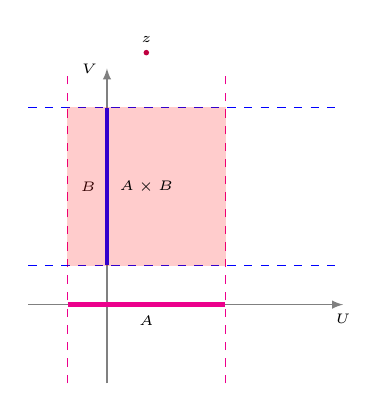
\begin{tikzpicture}[every node/.style={color=black,font={\tiny}}]
            \draw[thin, -latex, gray] (-1,0) -- (3,0) node[below] {$U$};
            \draw[thin, -latex, gray] (0, -1) -- (0,3) node[left] {$V$};
            % Conjunto A
            \draw[dashed, magenta] (-0.5, -1 ) -- (-0.5,3) node[left] {};
            \draw[dashed, magenta] (1.5, -1 ) -- (1.5,3) node[left] {};
            \draw[ultra thick, magenta] (-0.5, 0) -- (1.5,0) node[midway, below] {$A$};

            % Conjunto B
            \draw[dashed, blue] (-1,0.5  ) -- (3,0.5) node[left] {};
            \draw[dashed, blue] (-1,2.5  ) -- (3,2.5) node[left] {};
            \draw[ultra thick, blue] (0, 0.5) -- (0,2.5) node[midway, left] {$B$};

            \filldraw[opacity=0.2, red] (-0.5,0.5) rectangle (1.5,2.5) node (rectangulo) [midway] {};
            \node (conjunto) at (rectangulo.center) {\tiny\blue{$A \times B$}};

            \fill[purple] (0.5, 3.2) circle (1pt) node[above] {\purple{$z$}};
          \end{tikzpicture}
          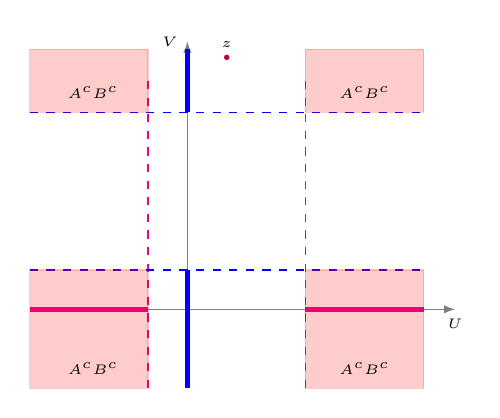
\begin{tikzpicture}[every node/.style={color=black,font={\tiny}}]
            \draw[thin, -latex, gray] (-1,0) -- (3.4,0) node[below] {$U$};
            \draw[thin, -latex, gray] (0, -1) -- (0,3.4) node[left] {$V$};

            % Conjunto A^c
            \draw[dashed, magenta] (-0.5, -1 ) -- (-0.5,3) node[left] {};
            \draw[dashed, magenta] (1.5, -1 ) -- (1.5,3) node[left] {};
            \draw[ultra thick, magenta] (-0.5, 0) -- (-2,0) node[midway, below]{};
            \draw[ultra thick, magenta] (1.5, 0) -- (3,0) node[midway, below]{};

            % Conjunto B^c
            \draw[dashed, blue] (-2,0.5  ) -- (3,0.5) node[left] {};
            \draw[dashed, blue] (-2,2.5  ) -- (3,2.5) node[left] {};
            \draw[ultra thick, blue] (0, 2.5) -- (0,3.3) node[midway, left] {};
            \draw[ultra thick, blue] (0, 0.5) -- (0,-1) node[midway, left] {};

            % Shading notA and notB intersection
            \filldraw[opacity=0.2, red] (-2,-1) rectangle (-0.5,0.5);
            \filldraw[opacity=0.2, red] (-2,2.5) rectangle (-0.5,3.3);
            \filldraw[opacity=0.2, red] (1.5,-1) rectangle (3,0.5);
            \filldraw[opacity=0.2, red] (1.5,2.5) rectangle (3,3.3);

            \node at (-1.2, -0.75) {\tiny\red{$A^c \inter B^c$}};
            \node at (2.25, -0.75) {\tiny\red{$A^c \inter B^c$}};
            \node at (-1.2, 2.75) {\tiny\red{$A^c \inter B^c$}};
            \node at (2.25, 2.75) {\tiny\red{$A^c  \inter B^c$}};

            \fill[purple] (0.5, 3.2) circle (1pt) node[above] {\purple{$z$}};

          \end{tikzpicture}
        \end{center}

  \item \hypertarget{teoria-1:relaciones}{\textit{Relaciones $\relacion$:}}\par
        \begin{itemize}[label=\tiny\faIcon{yin-yang}]
          \item
                \textit{Definición de relación: }\par
                Sean $A$ y $B$ conjuntos. Una relación $\relacion$ de $A$ en $B$ es un suconjunto
                cualquiera $\relacion$ del producto cartesiano $A \times B$. Es decir $\relacion$ es una relación
                de $A$ en $B$ si $\relacion \en \partes(A \times B)$.
          \item
                \textit{Definición de relación en un conjunto: }\par
                Sea $A$ un conjunto. Se dice que $\relacion$ en $A$ cuando $\relacion \subseteq A \times A$.
        \end{itemize}

  \item \hypertarget{teoria-1:prop-relaciones}{\textit{Propiedades destacables de una $\relacion$:}}\par
        \begin{enumerate}[label=\tiny\faIcon{poop}]
          \item  \textit{Reflexiva}: $(x, x) \en \relacion \paratodo x \en A$ o $x \relacion x.\, \paratodo x \en A$. Gráficamente,
                cada elemento tiene que tener un bucle.
                \begin{tikzpicture}[baseline=0, >=Latex, draw=Aquamarine]
                  \node[](a) {$\bullet$} edge [in=0,out=90,loop] ();
                  \node[] at (a.west) {$x$};
                \end{tikzpicture}

          \item  \textit{Simétrica}: $(x, y) \en \relacion$, entonces el par $(y, x) \en \relacion$,
                también si $\paratodo x, y \en A, x\relacion y \entonces y \relacion x$.
                Gráficamente tiene que haber un ida y vuelta en cada elemento de la relación.
                \begin{tikzpicture}[baseline=-10, >=Latex, draw=Aquamarine]
                  \node[] (x) {$\bullet$};
                  \node[] at (x.west) {$x$};
                  \node[below right =0.2 of x] (y) {$\bullet$};
                  \node[] at (y.south east) {$y$};
                  \draw[->, bend left=1cm] (x.center) to (y);
                  \draw[->, bend left=1cm] (y.center) to (x);
                \end{tikzpicture}

          \item  \textit{Antisimétrica}: $(x, y) \en \relacion$, con $x \distinto y$ entonces el par $(y, x) \notin \relacion$, también se puede pensar
                como $\paratodo x,y \en A, x\relacion y$ e $ y \relacion x \entonces x = y$.
                Gráficamente \textbf{no} tiene que haber ningún ida y vuelta en el gráfico. Solo en una dirección.
                \begin{tikzpicture}[baseline=-10, >=Latex, draw=Aquamarine]
                  \node[] (x) {$\bullet$};
                  \node[] at (x.west) {$x$};
                  \node[below right =0.2 of x] (y) {$\bullet$};
                  \node[] at (y.south east) {$y$};
                  \draw[->] (x.center) to (y.center);
                \end{tikzpicture}

          \item  \textit{Transitiva}: Para toda terna $x, y, z \en A$ tales que $(x, y) \en \relacion$ e $(y,z) \en \relacion$,
                se tiene que $(x, z) \en \relacion$.
                Otra manera sería si $\paratodo x, y, z \en A$, $x \relacion y$ e $y \relacion z \entonces x\relacion z$.
                Gráficamente tiene que haber flecha directa entre las puntas de cualquier camino que vaya por más de dos nodos.
                \begin{tikzpicture}[baseline=0, >=Latex, draw=Aquamarine]
                  \node[] (x) {$\bullet$};
                  \node[] at (x.north east) {$x$};
                  \node[below right = 0.6cm of x] (y) {$\bullet$};
                  \node[] at (y.north east) {$y$};
                  \node[below right = 0.6cm of y] (z) {$\bullet$};
                  \node[] at (z.north east) {$z$};

                  \draw[->, bend left] (x.center) to (y.center);
                  \draw[->, bend left] (y.center) to (z.center);
                  \draw[->,magenta, bend right]
                  (x.center)
                  to node[midway,below left] {atajo}
                  (z.center);
                \end{tikzpicture}
        \end{enumerate}
  \item
        \begin{itemize}[label=\tiny\faIcon{poo}]
          \item \textit{Relación de equivalencia}: La relación debe ser reflexiva, simétrica y transitiva.
          \item \textit{Relación de orden}: La relación debe ser reflexiva, antisimétrica y transitiva.
        \end{itemize}

  \item \hypertarget{teoria-1:funciones}{\textit{Funciones $f$:}}

        \begin{itemize}[label=\tiny\faIcon{poo}]
          \item
                Sean $A$ y  $B$ conjuntos, y sea $\relacion$ de $A$ en $B$. Se dice que
                $\relacion$ es una \textit{función} cuando todo elemento $x \en A$ está relacionado con algún
                $y \en B$, y este elemento $y$ es único. Es decir:
                $$\begin{array}{l}
                    \paratodo x \en A, \existe!\, y \en B \talque x \relacion y \\
                    \paratodo x \en A, \existe\, y \en B \talque x\relacion y,
                  \end{array}
                $$
                si  $y, z \en B \text{ son tales que } x \relacion y \ytext x \relacion z \entonces y = z$.

                \begin{itemize}[label=\tiny\faIcon{poop}]
                  \item Dada una función $f:\, A\,(dominio) \to B\,(codominio)$
                        el conjunto \textit{imagen} es:
                        $$
                          \im(f)= \set{y \en B : \existe x \en A \talque f(x) = y}
                        $$

                  \item \textit{Propiedades destacables de una $f$:}
                        \begin{itemize}[label=\tiny\faIcon{spider}]
                          \item \textit{inyectiva:} si $\paratodo x, x' \en A \text{ tales que } f(x) = f(x')$ se tiene que $ x = x'$
                          \item \textit{sobreyectiva:} si $\paratodo y \en B, \existe x \en A \text{ tal que } f(x) = y.\: f\text{ es sobreyectiva si } \im(f) = B$
                          \item \textit{biyectiva:} Cuando es \textit{inyectiva} y \textit{sobreyectiva}.
                        \end{itemize}

                  \item \textit{Composición de funciones:}\par
                        $A, B, C$ conjuntos y $f: A \to B \to C,\, g: B \to C$ funciones. Entonces la \textit{composición} de $f$ con $g$, que se nota:
                        $$
                          g \comp f = g(f(x)),\, \paratodo x \en A,
                        $$
                        resulta ser una función $g \comp f$ de $A$ en $C$.

                  \item $f$ es biyectiva cuando $f\inv : B \to A$ es la función que satisface que:\par
                        $$
                          \paratodo y \en B: f\inv(y) = x \sisolosi f(x) = y
                        $$
                \end{itemize}
        \end{itemize}
\end{itemize}
